%++++++++++++++++++++++++++++++++++++++++
\documentclass[a4paper,11pt]{article}
\usepackage{url}
\usepackage{hyperref}
\usepackage{fullpage}
\usepackage{booktabs}
\usepackage{graphicx}
\usepackage{wrapfig}
\usepackage{caption}
\usepackage{float}
\usepackage{subcaption}
\usepackage{enumerate}
\usepackage{color}
\usepackage{capt-of}
\usepackage{todonotes}
\usepackage{geometry}
 \geometry{
   a4paper,
   total={170mm,257mm},
   left=20mm,
   right=20mm,
   top=15mm,
 }
\usepackage{indentfirst}
  \setlength{\parindent}{0.5em}
  \setlength{\parskip}{0.1em} 
\usepackage{tabularx} % extra features for tabular environment
\usepackage{amsmath}  % improve math presentation
\newcommand{\Test}[1]{\expandafter\hat#1}
\usepackage{graphicx} % takes care of graphic including machinery
\hypersetup{
    colorlinks=true,       % false: boxed links; true: colored links
    linkcolor=blue,        % color of internal links
    citecolor=blue,        % color of links to bibliography
    filecolor=magenta,     % color of file links
    urlcolor=blue
}

% other packages
\usepackage{listings} % code listings
\lstset{framextopmargin=0pt,frame=lines}
\lstset{
    basicstyle=\footnotesize\ttfamily,
    breaklines=true,
    tabsize=4,
    keepspaces=true,
    columns=flexible,
    % backgroundcolor=\color[gray]{0.9},
    frame=single
}

\usepackage{todonotes}

%++++++++++++++++++++++++++++++++++++++++

\begin{document}

\title{
    System Identification \\
    CE-2: Frequency domain methods
}
\author{Camilla Carta \\ Michael Spieler}
\date{\today}
\maketitle

\section{Frequency domain Identification (Periodic signal)}

We apply a signal that contains several frequency components, such as a PRBS signal. Then we divide element-wise the Fourier transform of the output signal by the Fourier transform of the input signal. 
\begin{equation*}
G(e^{j\omega}) =  \frac{Y(e^{j\omega})}{U(e^{j\omega})}
\end{equation*}

To reduce the noise, we average over 16 periods before the division, leaving us with periods of length 127.

\begin{figure}[H]
	\centering
    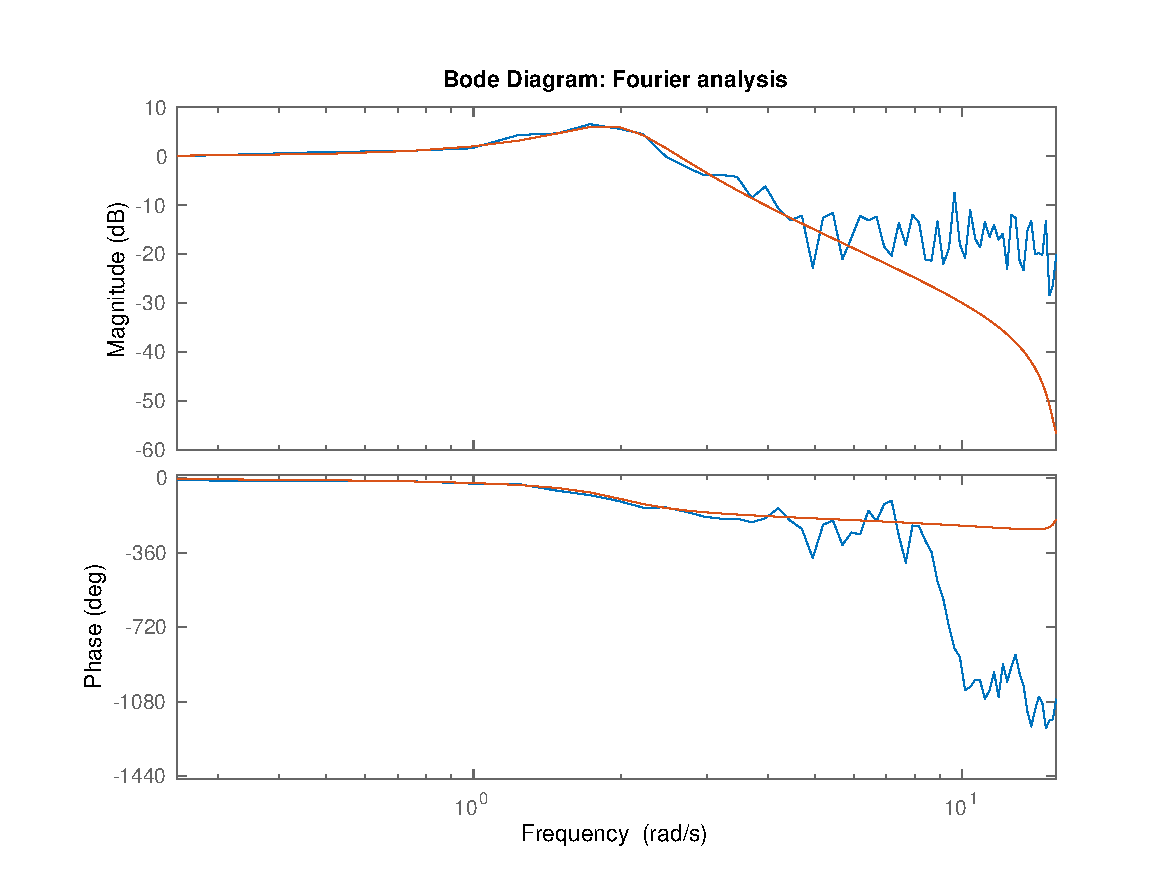
\includegraphics[height=9cm]{images/ce2_1_fourier_analysis}
    \caption{Frequency response using Fourier analysis}
    \label{fig:fourier_analysis}
\end{figure}

The Fourier analysis results in a relatively good reconstruction for lower frequencies while getting relatively noisy at high frequencies.

\begin{lstlisting}[language=Matlab,numbers=left,caption=Fourier analysis method,label=lst:fourier_analysis_code]
% input signal
saturation = 0.5;
noiseVariance = 0.1;

N_PERIODS = 16;
PERIOD_LEN = 2^7-1;
u = 0.5*prbs(7,N_PERIODS);
Te = 0.2; % sample time
N = length(u);
sim_time = N*Te;

% simulation
simin = struct();
simin.signals = struct('values', u);
simin.time = linspace(0,N*Te, N);
sim('ce1_1_sim')

%% Fourier transform
omega_s = 2*pi/Te;
avg = zeros(PERIOD_LEN,1);
for i = 1:PERIOD_LEN:N
    sig = simout(i:i+PERIOD_LEN-1);
    avg = avg + fft(sig);
end
freq = [];
for i = 0:PERIOD_LEN-1
   freq = [freq; i*omega_s/127];
end

Y = avg / N_PERIODS;
U = fft(u(1:PERIOD_LEN));
%% Reconstruction

Gr = Y ./ U;

NYQUIST_INDEX = round(PERIOD_LEN/2);
freq = freq(1:NYQUIST_INDEX);
Gr = Gr(1:NYQUIST_INDEX);

model = frd(Gr, freq, Te);

% true system
G = tf([4],[1 1 4]);
Z = c2d(G, Te, 'zoh');

% plot
figure
hold on
bode(model)
bode(Z,freq)
title('Bode Diagram: Fourier analysis')
hold off
\end{lstlisting}

\section{Frequency domain Identification (Random signal)}
We apply a PRBS signal of length 1024 to the simulation using a time step $Te = 0.2$.

When the random input signal $u(k)$ is uncorrelated with the disturbance signal $d(k)$ then:

\begin{equation*}
R_{yu}(h) = g(h)*R_{uu}(h)
\end{equation*}
Taking the FT:
\begin{equation*}
\Phi_{yu}(\omega) = G(e^{j\omega})\Phi_{uu}(\omega)
\end{equation*}
Thus we can reconstruct the frequency response by dividing the FTs of cross correlation $R_{yu}$ and autocorrelation $R_{uu}$.
\begin{equation*}
G(e^{j\omega}) = \frac{\Phi_{yu}(\omega)}{\Phi_{uu}(\omega)}
\end{equation*}



Figure \ref{fig:bode_no_window} shows the spectral analysis method applied to the simulation output with a random (PRBS) input. We used the biased cross- and autocorrelation function estimates.

We observe that the estimation is relatively good until the peak at $1.9 rad/s$ after that it becomes noisy and the phase diverges.

\begin{figure}[H]
	\centering
    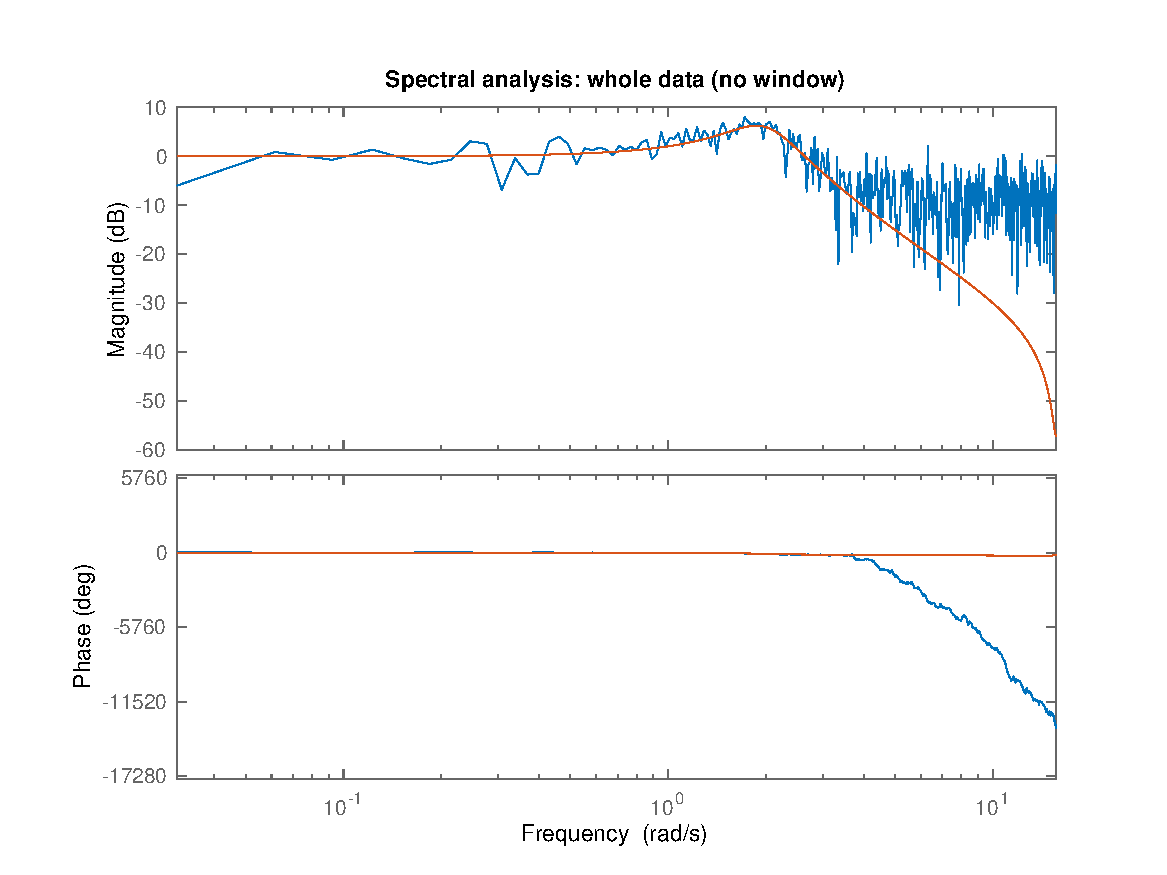
\includegraphics[height=9cm]{images/ce2_2_no_window}
    \caption{Spectral analysis method.}
    \label{fig:bode_no_window}
\end{figure}

\subsection*{Windowing}
To reduce the truncation error we use windowing, which is a weighting function in the time domain. The default window is a $rect(t)$ function which becomes a $sinc(\omega)$ in the Fourier domain. The side lobes introduce errors from other frequencies. We use a Hann window which has a bigger main lobe width (MLW) of $4\pi/N$ and a second lobe amplitude (SLA) of only 2.7\%.
The Hann window is defined as follows:
\begin{equation*}
f_{Hann}(t) =
\begin{cases}
0.5(1+cos(\frac{\pi t}{N})) & \text{for}\ t \in [-N,N] \\
0 & \text{elsewhere}
\end{cases}
\end{equation*}

Figure \ref{fig:bode_hann} shows the reconstruction using a Hann window of length 40. We observe that there is significantly less noise and the phase is more stable. Though the reconstruction has a lower peak at around $1.9rad/s$.

\begin{figure}[H]
	\centering
    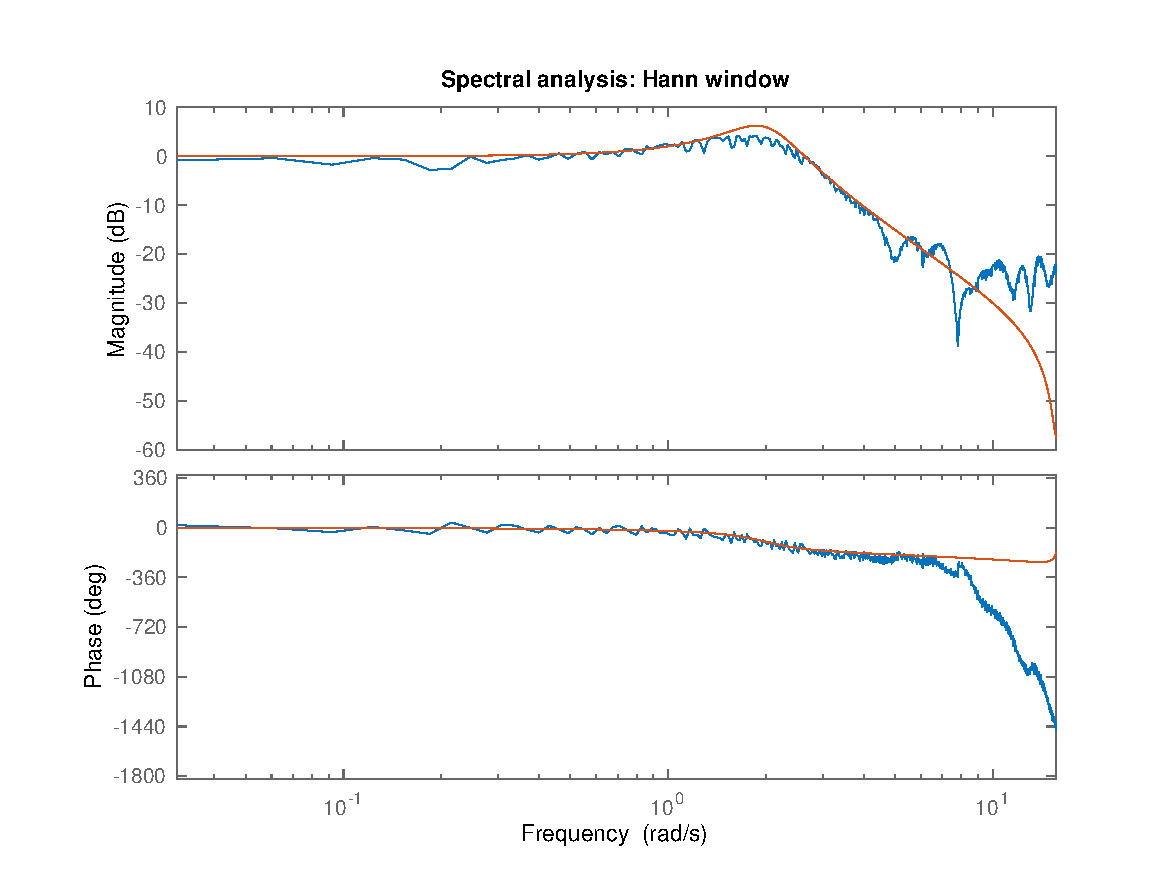
\includegraphics[height=9cm]{images/ce2_2_hann_window}
    \caption{Spectral analysis method with a Hann window.}
    \label{fig:bode_hann}
\end{figure}

Listing \ref{lst:spectral_analysis} shows the spectral analysis implementation in form of a Matlab function, allowing for optional windowing and selection of a biased or unbiased estimator of $R_{yu}$ and $R_{uu}$.

\begin{lstlisting}[language=Matlab,numbers=left,caption=spectral analysis,label=lst:spectral_analysis]
function model = spectral_analysis(y,u,Te,SCALEOPT,window)

N = length(u);

if nargin < 4
    SCALEOPT = 'biased';
end
if nargin < 5
    window = ones(N,1);
end

% correlation
Ryu = xcorr(y,u, SCALEOPT);
Ruu = xcorr(u,u, SCALEOPT);

Ryu = Ryu(N:end);
Ruu = Ruu(N:end);

% Windowing
padding = zeros(N - length(window), 1);
window = [window; padding];
Ryu = Ryu.*window;

% Reconstruction
Gr = fft(Ryu)./fft(Ruu);

omega_s = 2*pi/Te;
freq = 0:omega_s/N:(N-1)/N*omega_s;

NYQUIST_INDEX = round(N/2);
Gr = Gr(1:NYQUIST_INDEX);
freq = freq(1:NYQUIST_INDEX);

model = frd(Gr, freq, Te);
\end{lstlisting}

\subsection*{Averaging}

We can reduce the noise by splitting the data into multiple chunks and averaging over the FT of the cross- and autocorrelation estimates before dividing them.

Figure \ref{fig:bode_avg} shows the frequency response reconstruction using averaging over 8 parts.
In the left no window was applied and in the right we used a Hann window of length 40.
We observe a significant reduction of noise and more stable phase in respect to simple spectral analysis method.
When using a window the noise is slightly more reduced but we loose again amplitude at the peak at $1.9rad/s$.

\begin{figure}[H]
	\centering
    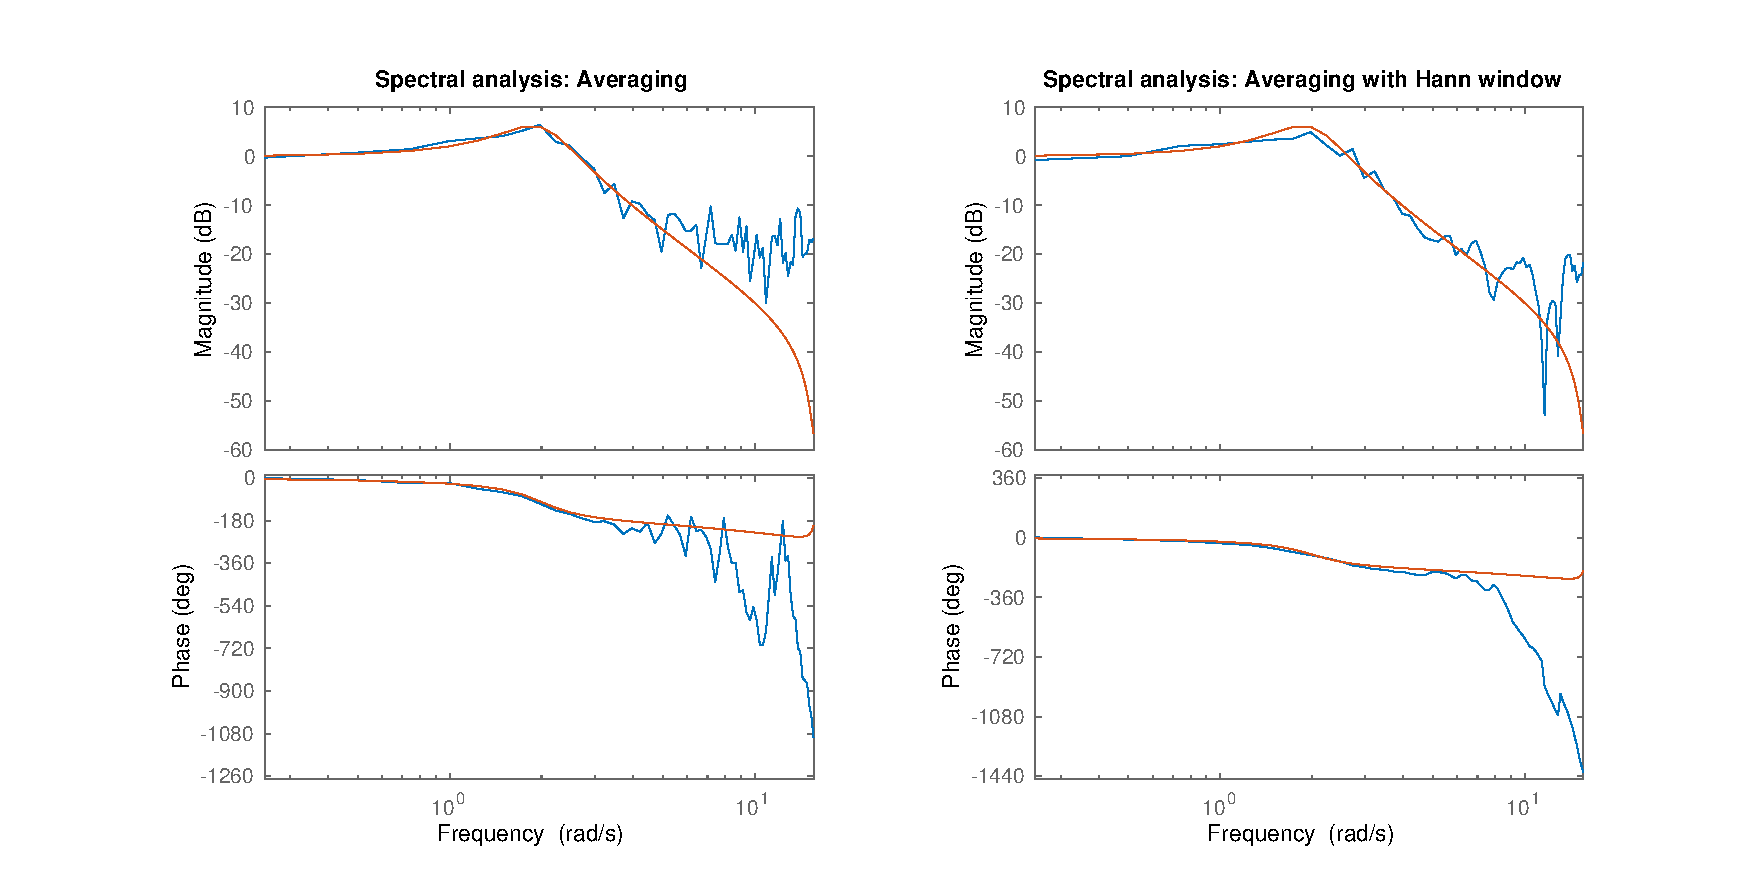
\includegraphics[height=9cm]{images/ce2_2_averaging}
    \caption{Spectral analysis method using averaging with and without windowing.}
    \label{fig:bode_avg}
\end{figure}

Listing \ref{lst:spectral_analysis_avg} shows the spectral analysis implementation with averaging in form of a Matlab function.

\begin{lstlisting}[language=Matlab,numbers=left,caption=spectral analysis avg,label=lst:spectral_analysis_avg]
function model = spectral_analysis_avg(y,u,Te,N_AVG,SCALEOPT,window)

N = floor(length(u)/N_AVG);

if nargin < 5
    SCALEOPT = 'biased';
end
if nargin < 6
    window = ones(N,1);
end
padding = zeros(N - length(window), 1);
window = [window; padding];

fft_Ryu = zeros(N,1);
fft_Ruu = zeros(N,1);
for i = 0:N_AVG-1
    % split into chunks
    yc = y(i*N + 1:(i+1)*N);
    uc = u(i*N + 1:(i+1)*N);

    % correlation
    Ryu = xcorr(yc,uc, SCALEOPT);
    Ruu = xcorr(uc,uc, SCALEOPT);

    Ryu = Ryu(N:end);
    Ruu = Ruu(N:end);

    % windowing
    Ryu = Ryu .* window;

    % averaging
    fft_Ryu = fft_Ryu+fft(Ryu);
    fft_Ruu = fft_Ruu+fft(Ruu);
end

% Reconstruction
Gr = fft_Ryu./fft_Ruu;

omega_s = 2*pi/Te;
freq = 0:omega_s/N:(N-1)/N*omega_s;

NYQUIST_INDEX = round(N/2);
Gr = Gr(1:NYQUIST_INDEX);
freq = freq(1:NYQUIST_INDEX);

model = frd(Gr, freq, Te);
\end{lstlisting}

\subsection*{Unbiased estimator of cross- and autocorrelation function}

Figure \ref{fig:bode_unbiased} compares results using biased and unbiased estimations of the cross-correlation and autocorrelation functions used in the spectral analysis method. We observe that the unbiased estimator is more noisy and corresponds less to the true model.

\begin{figure}[H]
	\centering
    \hspace*{-2.5cm}
    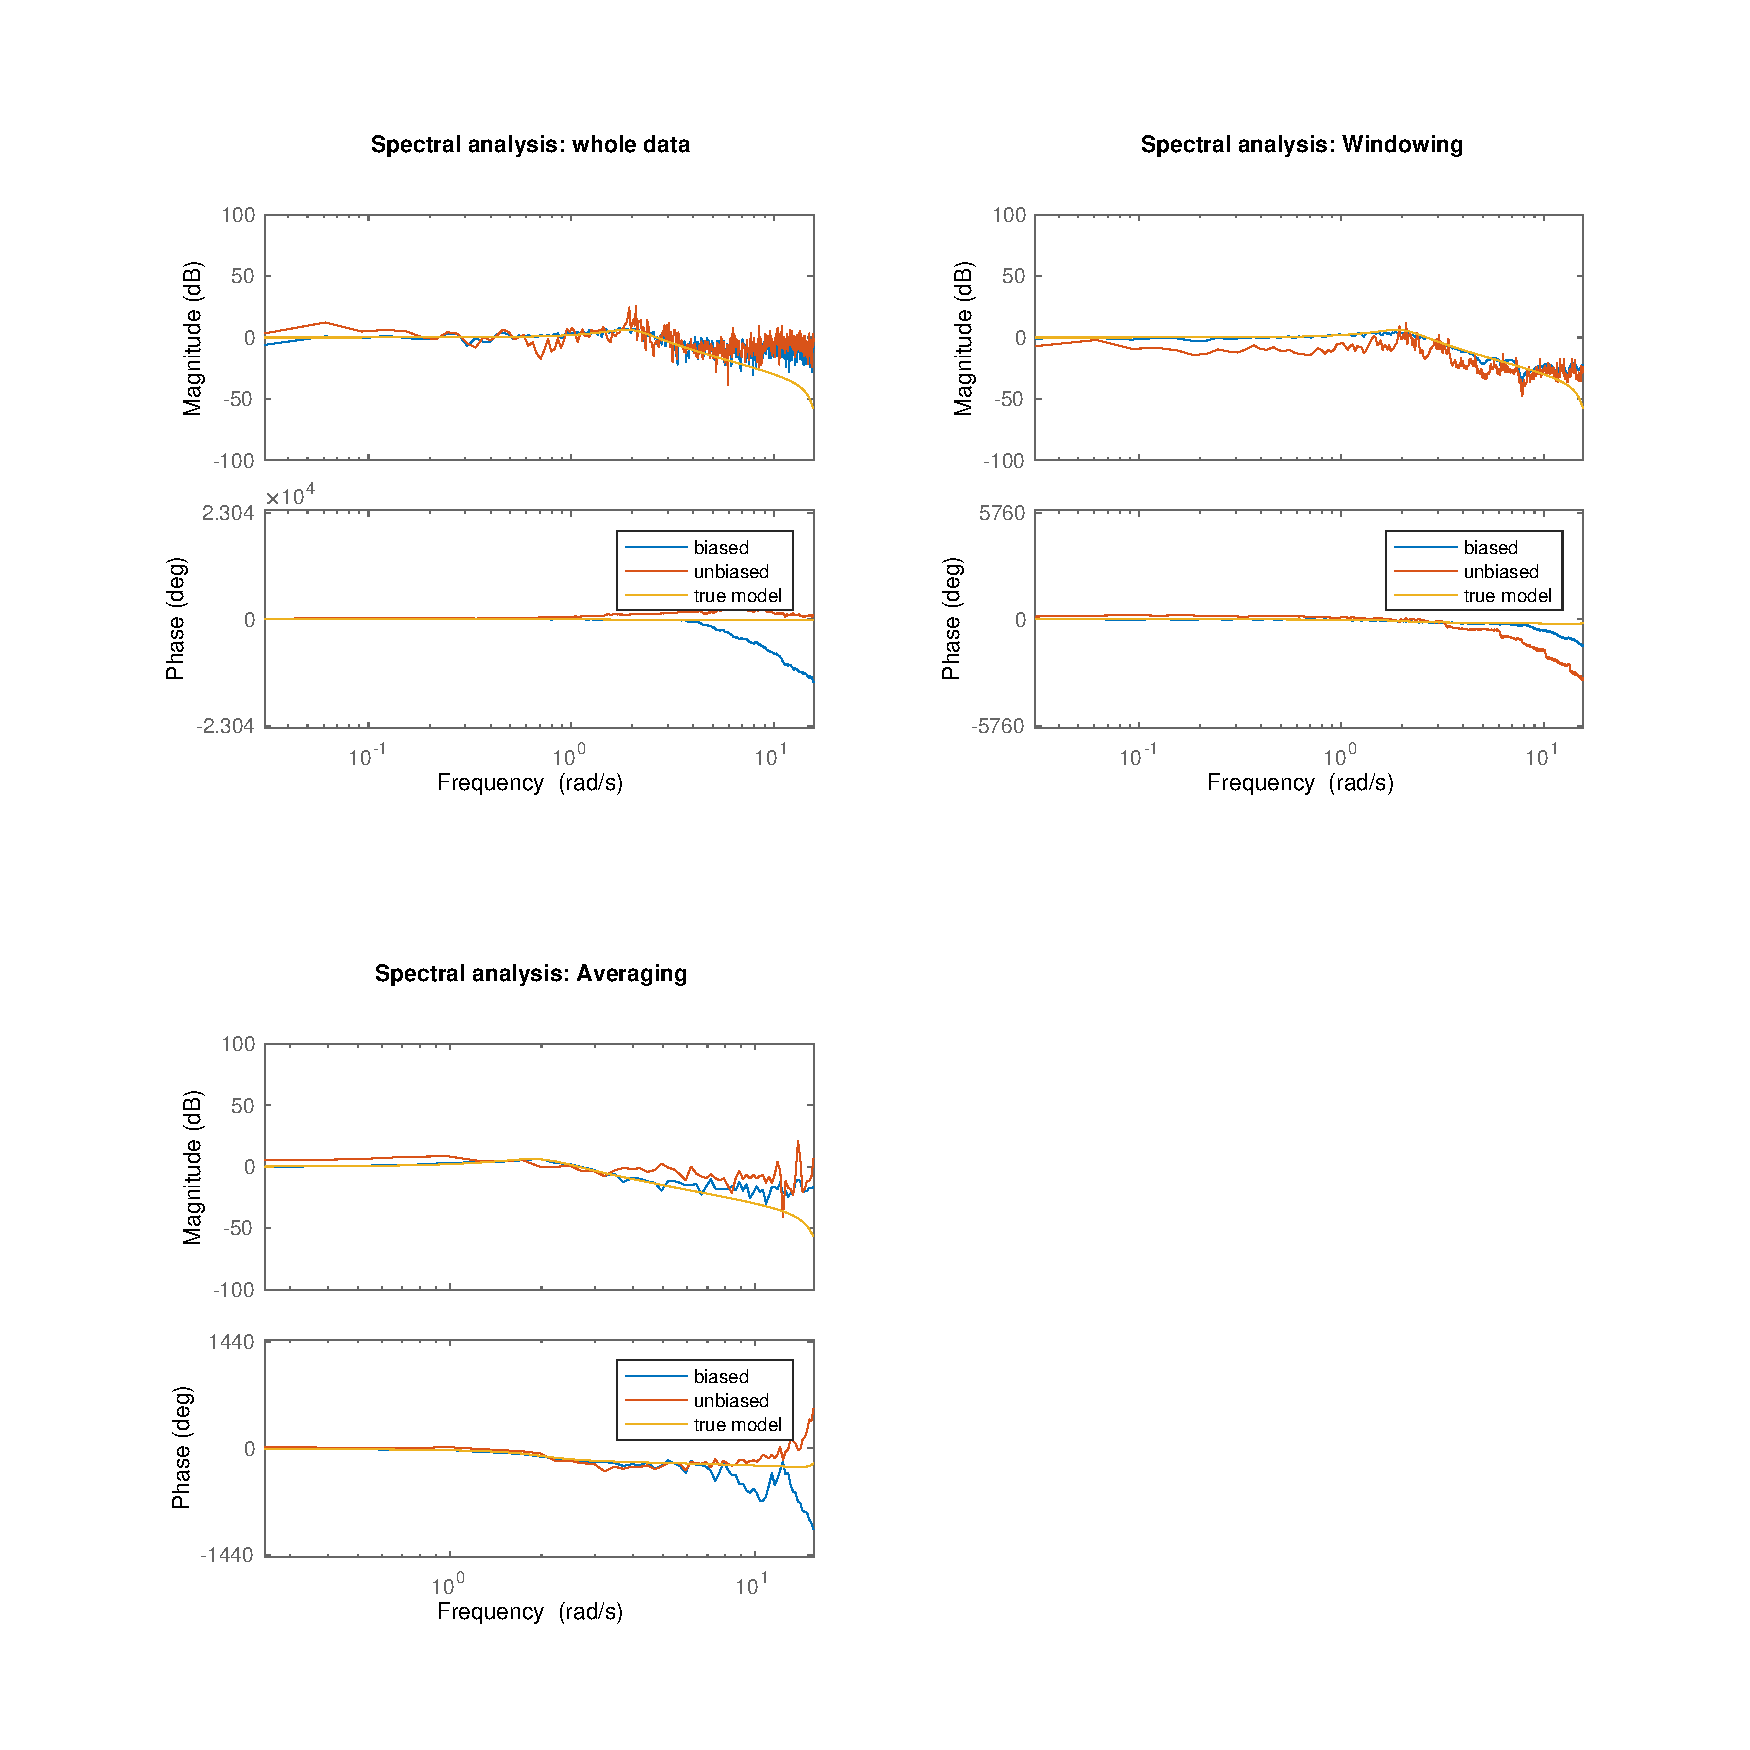
\includegraphics[height=1.3\textwidth]{images/ce2_2_unbiased}
    \caption{Comparing spectral analysis method based on biased and unbiased estimations of the correlation functions.}
    \label{fig:bode_unbiased}
\end{figure}

\section{Simulation and plot generation code}
\begin{lstlisting}[language=Matlab,numbers=left,caption=Spectral analysis method,label=lst:spectral_analysis_code]
% simulation parameters
saturation = 0.5;
noiseVariance = 0.1;

% input signal
u = 0.5*prbs(10,1);
PERIOD_LEN = length(u);
Te = 0.2; % sample time
N = length(u);
sim_time = N*Te;

% simulation
simin = struct();
simin.signals = struct('values', u);
simin.time = linspace(0,N*Te, N);
sim('ce1_1_sim')
y = simout;

% true system
G = tf([4],[1 1 4]);
Z = c2d(G, Te, 'zoh');


%% Spectral analysis method
model = spectral_analysis(y,u,Te,'biased');

% Windowing
hann = @(M) 0.5+0.5*cos(pi*[0:M-1]'/(M-1));
hamming = @(M) 0.54+0.46*cos(pi*[0:M-1]'/(M-1));

window = hann(40);
model_hann = spectral_analysis(y,u,Te,'biased',window);

% Bode plot
figure
hold on
bode(model)
bode(Z,model.Frequency)
title('Spectral analysis: whole data (no window)')
hold off

figure
hold on
bode(model_hann)
bode(Z,model_hann.Frequency)
title('Spectral analysis: Hann window')
hold off

%% Averaging
N_AVG = 8;

% averaging without window
model = spectral_analysis_avg(y,u,Te,N_AVG,'biased');

% averaging with Hann window
window = hann(40);
model_hann = spectral_analysis_avg(y,u,Te,N_AVG,'biased',window);

figure
subplot(1,2,1)
hold on
bode(model)
bode(Z,model.Frequency)
title('Spectral analysis: Averaging')
hold off
subplot(1,2,2)
hold on
bode(model_hann)
bode(Z,model.Frequency)
title('Spectral analysis: Averaging with Hann window')
hold off


%% unbiased plots
figure
subplot(2,2,1)
hold on
model_biased = spectral_analysis(y,u,Te,'biased');
model_unbiased = spectral_analysis(y,u,Te,'unbiased');
bode(model_biased)
bode(model_unbiased)
bode(Z,model_biased.Frequency)
title('Spectral analysis: whole data')
legend('biased','unbiased','true model')
hold off

window = hann(40);
subplot(2,2,2)
hold on
model_biased = spectral_analysis(y,u,Te,'biased',window);
model_unbiased = spectral_analysis(y,u,Te,'unbiased',window);
bode(model_biased)
bode(model_unbiased)
bode(Z,model_biased.Frequency)
title('Spectral analysis: Windowing')
legend('biased','unbiased','true model')
hold off

subplot(2,2,3)
hold on
model_biased = spectral_analysis_avg(y,u,Te,N_AVG,'biased');
model_unbiased = spectral_analysis_avg(y,u,Te,N_AVG,'unbiased');
bode(model_biased)
bode(model_unbiased)
bode(Z,model_biased.Frequency)
title('Spectral analysis: Averaging')
legend('biased','unbiased','true model')
hold off
\end{lstlisting}


\end{document}
